\section{Operating System Security}

\begin{itemize}
    \item OS controls access to resources
    \item OS schedules processes
    \item OS offers security to processes
\end{itemize}

\begin{itemize}
    \item safety: Users can perform only authorized operations
    \item least privilege: Processes perform only their necessary operations
    \item MLS: Operations can only permit information to be written to more secret levels.
\end{itemize}

\paragraph{Security Goals}
\begin{itemize}
    \item Secrecy: who can read what files?
    \item Integrity: who can write to what files?
    \item Availability: what processes can consume storage/CPU/memory?
\end{itemize}

\paragraph{Trust Model}
The set of software and data upon which the system depends for correct enforcement of system security goals. Ideally as little as absolutely necessary. Also known as Trusted Computing Base TCB.\\
\\
Linux TCB: Kernel, modules, shell, system tools, X server, etc.

\paragraph{Threat Model}
Set of operations that an attacker may use to compromise. 
\textbf{Compromise: }violate a security goal by finding a
vulnerability

\subsection{Access Control}
The selective restriction of access to a resource. Whether to allow requests from multiple subjects to perform operations on objects.\\
\\
The security requirements of an OS are defined by
its protection system
\begin{itemize}
    \item A protection system is comprised of a protection
    state and protection state operations.
    \item Protection state - Operations that subjects can
    perform on objects
    \item Protection state operations - Enable modification
    of state
\end{itemize}

\paragraph{Access Matrix}
Consists of a set of subjects s a set of objects o a set of operations op and a function ops(s, o), which determines the operations that subj s can perform on object o. Matrix can be stored by row or column:
\begin{itemize}
    \item[-]By column: Access control list (ACL) stored with resource.
    \item[-]By row: Capability of a given process or user
\end{itemize}

\paragraph{Unix File Protection: ACL (by column)}
\begin{itemize}
    \item Subjects: owner, group, others
    \item Operations: read (r), write (w), execute (x)
    \item rights are stored with the target object to be accessed.
\end{itemize}

\paragraph{Page Table: Capability (by row)}
Page Tables define the access domain, access rights are stored with the accessor.

\paragraph{Capabilities vs ACLs}
slide 37

\paragraph{MAC and DAC}
\begin{itemize}
    \item DAC: A protection system that permits untrusted processes to modify the protection state is called a discretionary access control system. DAC works if all processes are benign, and users make no mistakes (impossible). A subject with  certain access permissions can passs on exactly these permissions.
    \item MAC: A mandatory protection system can only be modified by trusted administrators via trusted software.
\end{itemize}

\paragraph{Reference Monitor}
\begin{itemize}
    \item Input: a request to perform a security-sensitive operation
    \item Output: binary response indicating whether the request is authorized by the policy
    \item Authorization module - the brains of the reference monitor. Must convert requests into a query that can be looked up in the policy store.
    \item Policy store - a database of protection state, labeling state and transition state. 
\end{itemize}

Secure OS definition: "A system with a reference monitor access enforcement mechanism that satisfies the requirements below:”
\begin{itemize}
    \item Complete mediation: must mediate all security-sensitive operations.
    \item Tamperproof: cannot be modified or disabled by untrusted processes.
    \item Verifiable: small enough to be subject to analysis. Simple policies are intuitive to verify, but complexity makes verification hard
\end{itemize}

\paragraph{Covert Channels}
Prevent unauthorized communication among processes. Protection models we discussed so far are not sufficient, processes can leak information through covert channels. Preventing Covert Channels slide 56.

\subsection{Linux Security Model}
Kernel enforces object permissions! \\
Notice the difference between kernel and superuser access\\
– Kernel processes can access anything\\
– Root processes can order the kernel to access anything\\

\paragraph{UNIX File Concepts}
\begin{itemize}
    \item files administered using i(index)nodes (control structure with key info of a single file (attributes, permissions, ..)
    \item Inode table/list for all files on a disk, copied to memory when disk mounted.
    \item Directories form a hirarchical tree : are a file of names and inode numbers.
    \item Linux treats everything as a file! Filesystem security very important.
\end{itemize}

\paragraph{Users and Groups}
\begin{itemize}
    \item User account: (user, uid) represents someone capable of using files (humans, processes).
    \item Group account: (group, gid) is a list of user-accounts
\end{itemize}

\paragraph{Using permissions}
\begin{itemize}
    \item A file has owner and group id (sometimes several)
    \item A process has owner and group id
    \item Kernel verifies permissions before executing system calls. (first uid and then gid are compared in this order!)
\end{itemize}

\paragraph{Linux Security Transactions}
\begin{itemize}
    \item A user executes a program (if it has permissions)
    \item When running the process normally runs as the user and group of the person or process that executed it.
    \item Whoever owns an object can set or change its permissions. • This is Linux DAC model’s real weakness: the system superuser account (“root”) can both take ownership and change the permissions of all objects in the system. It is not uncommon for processes and administrator-users to run with root privileges, in ways that provide attackers with opportunities to hijack those privileges.
\end{itemize}

\subsection{File Permissions}

\begin{itemize}
    \item Permissions: r, w, x
    \item For: Owner(User), Group, Others
    \item Directory permissions: r = list contents, w = create or delete files in dir, x = use anything in or change working dir to this dir (and read files if allowed by file permissions).
    \item The permissions are coded into the inodes
    \item Sticky bit: used on dirs to limit delete. If set must own file or dir to delete, other users cannot delete even if have write. (chmod + t)
    \item setuid bit: means program runs as owner no matter who executes it (chmod +s).
    \item setgid bit: means run as a memeber of the group which owns it. Only used on executable files, not shell scripts. Very dangerous!!
    \item setgid on dirs: causes any file created in a dir to inherit the dirs group.
    \item Changing passwords: Passwords are changed using the program /bin/passwd.
    \item Real UID = UID of the user running the program. Effective UID = UID of user with whose privileges the program runs.
    \item system calls slide 81
    \item Major problem in Unix is that everything is dependent on root and root has access to everything. Violation of principle of least privilege.
\end{itemize}

\subsection{SE Linux}
Linux uses DAC security model. But Mandatory Access Controls (MAC) imposes a global security policy on all users. 
\begin{itemize}
    \item users may not set controls weaker than policy.
    \item Normal admin done with accounts without authority to change the global sec policy
    \item But MAC systems have been hard to manage.
    \item In SELinux all access must be explicitly granted. Allows no access by default, regardless of the Linux user/group ID's
    \item No default superuser in SELinux, unlike root in standard Linux.
\end{itemize}{}

\paragraph{Role Based Access Control (RBAC)}
\begin{itemize}
    \item Rules specify Roles a user may assume
    \item other rules specify circumstances when a user may transition from one role to another.
\end{itemize}{}

\paragraph{Multi Level Security (MLS)}
\begin{itemize}
    \item Concerns handling of classified data (no read up, no write down)
    \item MLS is enforced via file system labeling
\end{itemize}{}

\paragraph{Security Contexts}
Each individual subject & object in SELinux is governed by a security context: 
\begin{itemize}
    \item User: (human or daemon) user labels on subjects specify accounts privileges. user labels on objects specify its owner.
    \item Role: like a group, assumed by users. Only one role per user.
    \item Domain (type): a sandbox being a combination of subj. and obj. that may interact with each other.
\end{itemize}{}
This model is called \textbf{Type Enforcement (TE)}. Subj Type can access obj. type to perform Operations on Obj.\\
\\
\paragraph{Decision Making in SELinux}
\begin{enumerate}
    \item access decisions: subj do things to obj that already exist, or create new things in expected domain.
    \item transition decisions: invocation of processes or creation of obj in different types (domains) than their parent domains. Transition must be authorized by SELinux policy. 
\end{enumerate}{}

\begin{figure}[h!]
    \centering
    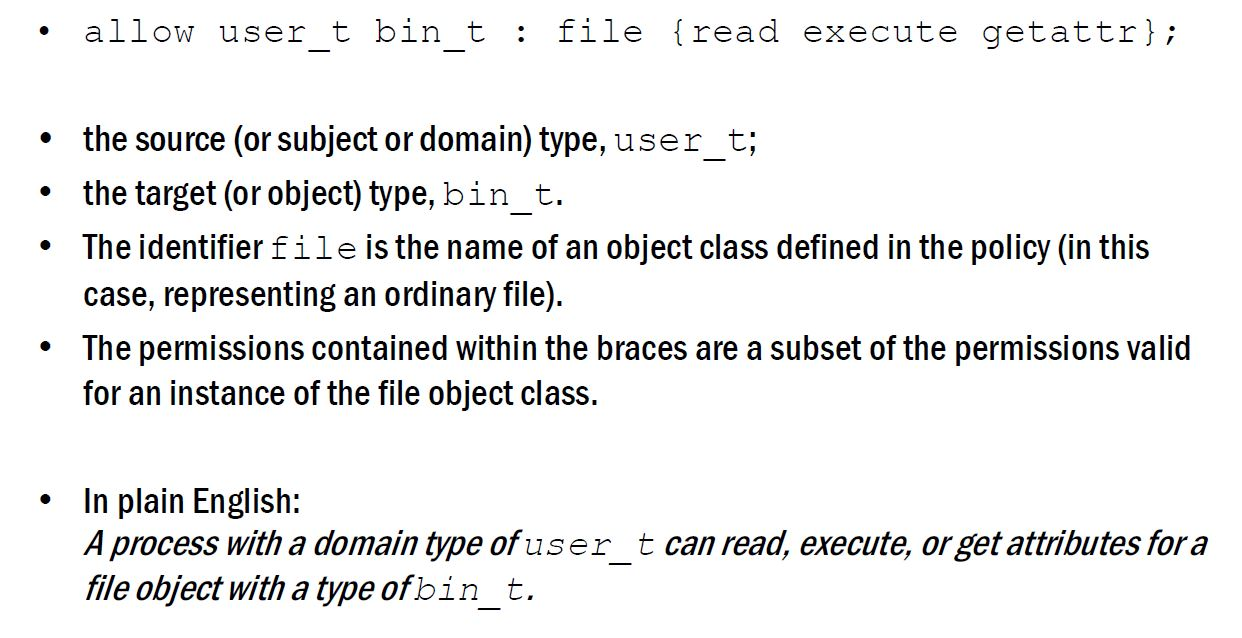
\includegraphics[scale=0.5]{Figures/SELinuxAC.JPG}
    \label{fig:Access Control}
\end{figure}

\paragraph{Why use Type Enforcement?}
\begin{itemize}
    \item It enables us to ensure that only the password program can access the shadow file, regardless of the user running the program (what normal unix AC cannot do)
    \item Problem slide 96ff. solution domain transitions!
    \item Providing for secure domain transition is analogous to the concept of setuid programs, but with the strength of type enforcement.
\end{itemize}{}

\paragraph{Domain Transition Rules}
all following three rules are necessary alone none is sufficient:
\begin{enumerate}
    \item The process new domain type has entrypoint access to an executable file type.
    \item The process current domain type has execute access to the entrypoint file type.
    \item The process current domain type has transition access to the new domain type.
\end{enumerate}{}

\subsection{Securing Commercial Operating Systems}
To make an OS secure, we need at least:
\begin{itemize}
    \item A reference monitor: system to monitor and enforce a security policy.
    \item Complete mediation: all security-sensitive operations must be directed to the reference monitor.
    \item Tamperproof: enforcement mechanism cannot be modified by untrusted processes.
    \item Verifiable: Small enough to audit, prove it satisfies goals.
\end{itemize}{}

\paragraph{Examples}
\begin{itemize}
    \item Compartments: Use multiple vm's to decouple different programs.
    \item microkernels: Make the actual kernel as small as possible.
\end{itemize}{}

\paragraph{Microkernels:}

\subsubsection{}{Building a Secure Linux}
Linux Security Module (LSM) Framework.\\
Basic Idea: 
\begin{itemize}
    \item Hook security functions and security data structures
    \item Allow registration and initialization of security modules (e.g. AppArmor , GRSec , SELinux)
    \item Limit performance overhead (especially when no module is loaded)
    \item SELinux: MAC for linux, using LSM.
\end{itemize}{}

\subsubsection{}{Android}
\begin{itemize}
    \item Built on top of the linux Kernel
    \item Several Security enhancements
    \item Security-Usability trade off.
    \item Java applications with native code components.
    \item Typically a single user. isolate apps not users.Each app has own Linux UID. (Apps cannot read eachothers files, memory and cannot exhaust all resources.
\end{itemize}

\paragraph{Android Permission Model:}
\begin{itemize}
    \item Restrict access to sensitive resources.
    \item Only accessible through OS (complete mediation)
    \item Application has to request permissions in manifest.
    \item Permission Enforcement: During critical system call.
    \item 
\end{itemize}{}

\paragraph{Application Signing}
\begin{itemize}
    \item Applications have to be signed by the developers.
    \item All Updates have to be signed with the same key.
    \item Applications signed by the same key can request same UID
    \item Signature matches app to developer who has to register with Google (Signature does not imply trustworthiniess)
    \item Google performs malware scan in market (bouncer) but numerous malware has made it past bouncer.
\end{itemize}{}

\subsubsection{Windows 10}
Allows different configurations to enhance security:
\begin{itemize}
    \item Enable Memory Protection: DEP, ASLR, ..
    \item UEFI Secure Boot
    \item Device Guard (contains whitelisted applications)
    \item BitLocker Drive Encryption
    \item AppContainer: Allows app sandboxing
    \item Windows Defender Antivirus
\end{itemize}{}



